\documentclass[aspectratio=1610]{beamer}
\usepackage[T1]{fontenc}
\usepackage{hardwrap}


\usetheme{wildcat}
\usetikzlibrary{shapes.geometric,arrows,positioning,fit,backgrounds}
\usepackage[backend=biber,style=authoryear]{biblatex}
\addbibresource{references.bib}

\title{Leveraging Nonlinear Systems Equation for Efficient Spam Email Detection}
\author{Maded by Group A}


\titlegraphic{
\includegraphics[scale=0.25]{680558}}

\tikzstyle{box} = [rectangle, draw, minimum width=2cm, minimum height=0.8cm, text centered, font=\footnotesize]
\tikzstyle{dashedbox} = [rectangle, draw, dashed, minimum width=3cm, minimum height=1.5cm, font=\footnotesize]
\tikzstyle{arrow} = [thick,->,>=stealth]


\begin{document}

%title page
\begin{frame}
\titlepage
\end{frame}

%slides 1 Group member
\begin{frame}{Group Members}
    \begin{center}
        \begin{tabular}{|c|l|}
            \hline
            \textbf{Matrix Number} & \textbf{Name} \\
            \hline
            S2191553 & Yerong Liu \\
            \hline
            U2100875 & HAFIZ AIMAN BIN SHAMSUL BAHARI \\
            \hline
            S2148250 & SOO WEE LIM \\
            \hline
            U2101770 & MUHAMMAD AIDIL SHAZWAN BIN MARZUKHI \\
            \hline
            S2190329 & Yulun Deng \\
            \hline
            S2109049 & SUMAIYA MUNTAREEN BILLAH \\
            \hline
        \end{tabular}
    \end{center}
\end{frame}






%slides 3 Introduction Section
\begin{frame}{Introduction}
    \frametitle{Introduction}
    \setlength{\baselineskip}{1.5em}
    Email remains a cornerstone of communication in the digital age, but its widespread use has led to the proliferation of spam emails, ranging from simple advertisements to malicious phishing and malware attempts. Traditional detection methods often fall short in addressing the complexity and adaptability of modern spam strategies. To tackle this challenge, integrating nonlinear systems equations into the \textbf{Backpropagation} process of machine learning models offers a promising solution. Nonlinear systems excel at capturing intricate patterns within data, enabling neural networks to better differentiate legitimate emails from spam while adapting to evolving threats. This approach enhances both detection accuracy and computational efficiency, providing a robust framework for large-scale email filtering.

\end{frame}


%Problem statement Section
\begin{frame}{Problem statement}
    \frametitle{Problem statement}
    With the rapid advancement of technology, the widespread adoption of large-scale AI models, and the increasing volume of spam, the prevalence of sophisticated spam has become a significant challenge. Traditional spam detection models often fail to effectively address the complexities of modern spam emails. As a result, there is a growing need for more complex and efficient spam processing models that can handle these advanced threats. To tackle this issue, leveraging nonlinear systems equations offers a promising approach to enhance the accuracy and efficiency of spam email detection.    
    
\end{frame}


%objectives Section
\begin{frame}{objectives}
    \frametitle{objectives}
    \begin{itemize}
        \item \textbf{Reducing Data Noise: }By filtering out spam, we can ensure that important communications are not lost among irrelevant messages, improving the efficiency of email usage.
        \item\textbf{Enhance Spam Detection Efficiency: }Incorporate nonlinear system equations into the backpropagation process and loss function calculations of machine learning models to improve the model's ability to efficiently identify and filter spam emails, even as spam strategies evolve.
        \item\textbf{Improve User Experience and System Adaptability: } Optimize the model to maintain computational efficiency while adapting to changing spam patterns, ensuring a seamless, responsive email filtering system that enhances the overall user experience.
    \end{itemize}
    
\end{frame}


%flow chart section
\begin{frame}{Flow Chart}
    \frametitle{Flow Chart }
    \begin{figure}
        \centering
        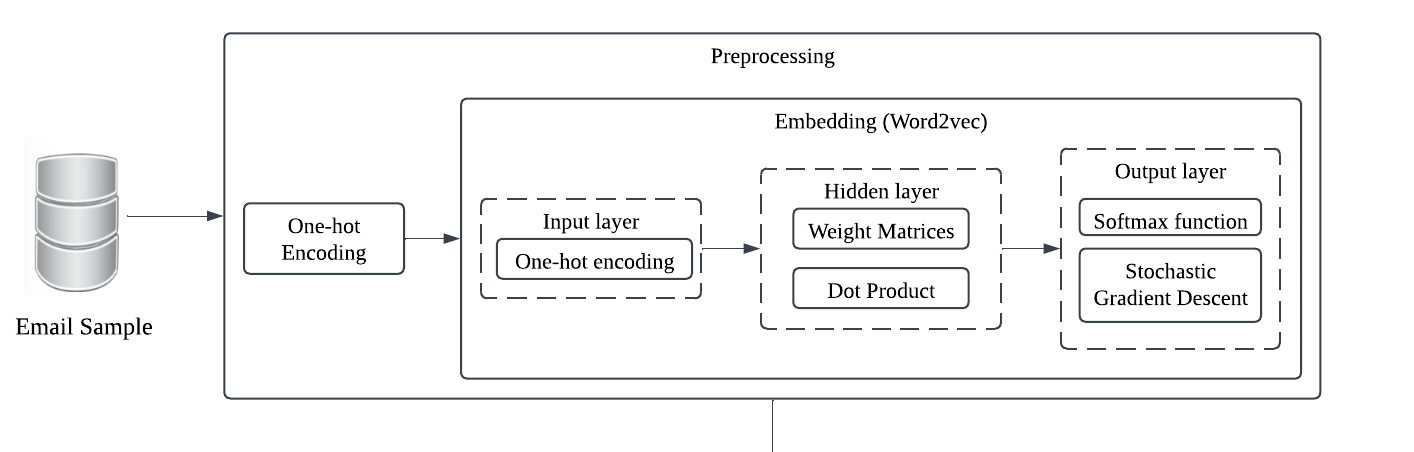
\includegraphics[width = 1.1\linewidth]{NA (1)[2]}
        \label{fig:figure}
    \end{figure}
    
\end{frame}

\begin{frame}{Flow Chart}
    \frametitle{Flow Chart}
        \begin{figure}
        \centering
        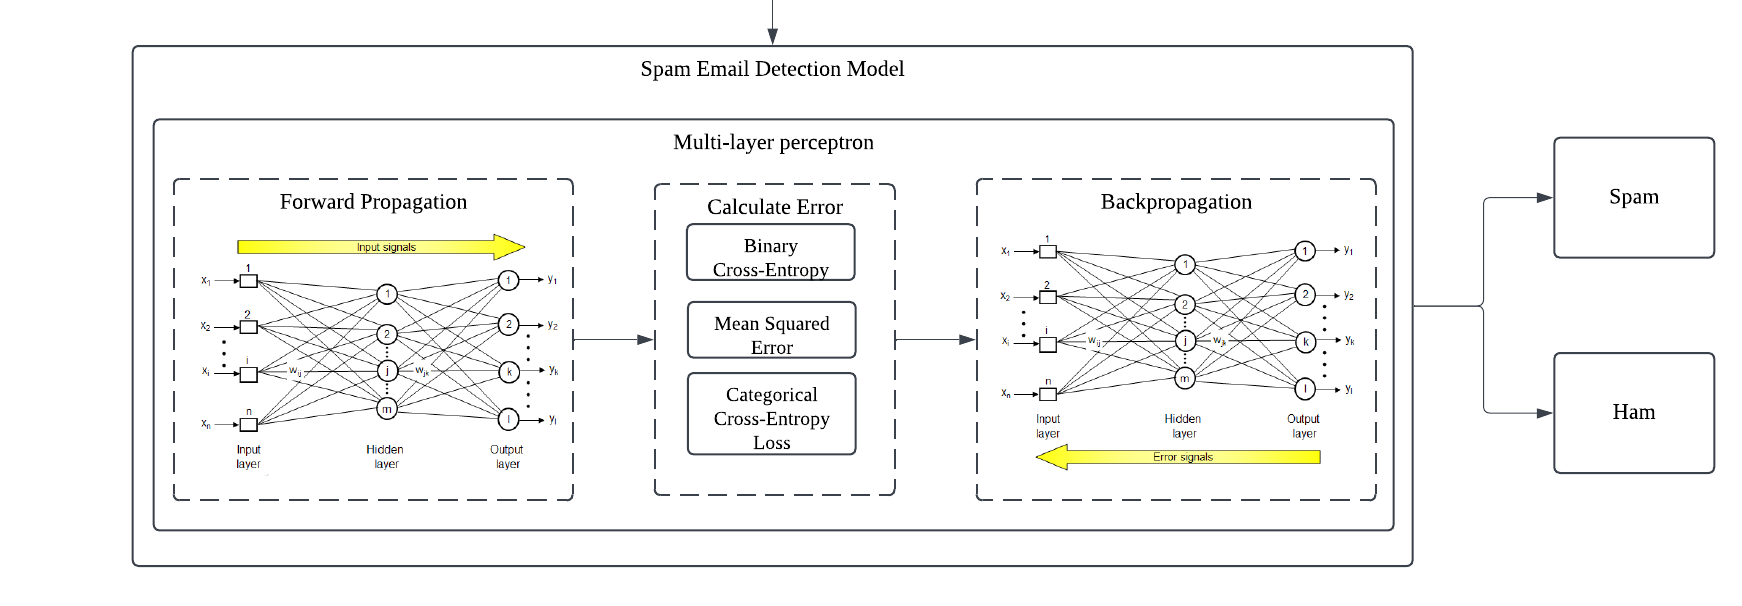
\includegraphics[width=1.1\linewidth]{D:/NA/NA (1)[1]}
        \caption{Detection Model}
        \label{fig:enter-label}
    \end{figure}
      
    
\end{frame}

\begin{frame}{Methodology}
    \frametitle{Methodology}
    \textbf{Backpropagation}\\
    \vspace{0.3cm}
    Backpropagation is enhanced by incorporating nonlinear system equations, which govern the behavior of activation functions like sigmoid or ReLU. These nonlinearities allow the model to capture complex patterns in data, improving tasks like spam detection. Nonlinear gradients enable precise adjustments to weights and biases, driving faster convergence and better performance throughout training.\\
    \vspace{0.5cm}
    \textbf{Loss Functions}\\
    \vspace{0.3cm}
    Nonlinear system equations in loss functions, such as Binary Cross-Entropy or Categorical Cross-Entropy, allow the model to handle outputs as probabilities. This nonlinearity ensures sensitive loss calculations, guiding the model towards better solutions. As training progresses, the loss decreases and stabilizes, enhancing the model’s ability to detect complex patterns, like spam, effectively and reliably.

\end{frame}

\begin{frame}
    \frametitle{Forward}
    Calculate the result of each node and pass to the next layer, when we reaching the final node, we’ll get the result. That’s the process of forward.
    \\The result $\boldsymbol{Z_1}$ is then passed through the ReLU activation function $\boldsymbol{f}$: 
    $\boldsymbol{Z_1} = \boldsymbol{X} \boldsymbol{W_1} + \boldsymbol{b_1}$, where 
    $\boldsymbol{f(x)} = \max(0, \boldsymbol{x})$ and $\boldsymbol{A_1} = \boldsymbol{f(Z_1)}$.
    \\The output from the hidden layer $\boldsymbol{A_1}$ is passed to the next layer. It is multiplied by the weight matrix $\boldsymbol{W_2}$ and added to the bias $\boldsymbol{b_2}$, resulting in $\boldsymbol{Z_2} = \boldsymbol{A_1}\boldsymbol{W_2} + \boldsymbol{b_2}$. The result $\boldsymbol{Z_2}$ is then passed through the sigmoid activation function $\boldsymbol{g(x)}$ to produce the final output $\boldsymbol{A_2}$, where 
    \[
    \boldsymbol{g(x)} = \frac{\boldsymbol{1}}{\boldsymbol{1} + \boldsymbol{e}^{-\boldsymbol{x}}}, \quad \boldsymbol{A_2} = \boldsymbol{g(Z_2)}.
    \]

    
    \begin{figure}
        \centering
        \begin{minipage}{0.6\textwidth}
            \centering
            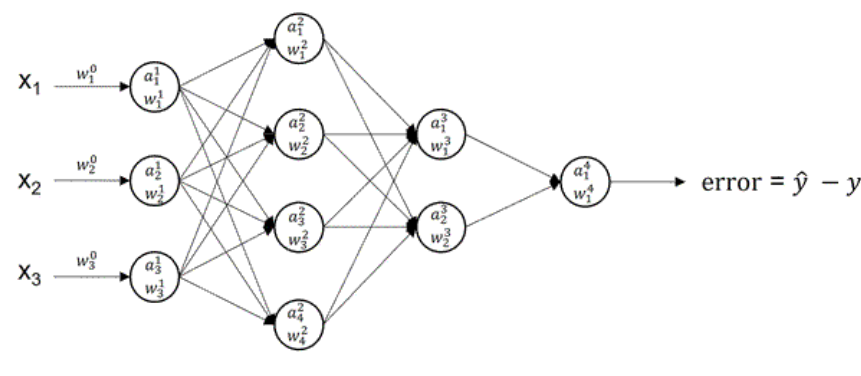
\includegraphics[width=\linewidth]{Forward.png}
        \end{minipage}%
        \hfill
        \begin{minipage}{0.35\textwidth}
            \centering
            \caption{Input Layer to Hidden Layer: input vector $X$, matrix $W$, bias $b_1$.}
            \label{fig:enter-label}
        \end{minipage}
    \end{figure}
\end{frame}


\begin{frame}
    \frametitle{Training: What is Backpropagation}
    Short for \textbf{"backward propagation of error"}, is an algorithm for supervised learning of artificial neural networks using gradient descent.
    \begin{figure}
        \begin{center}
            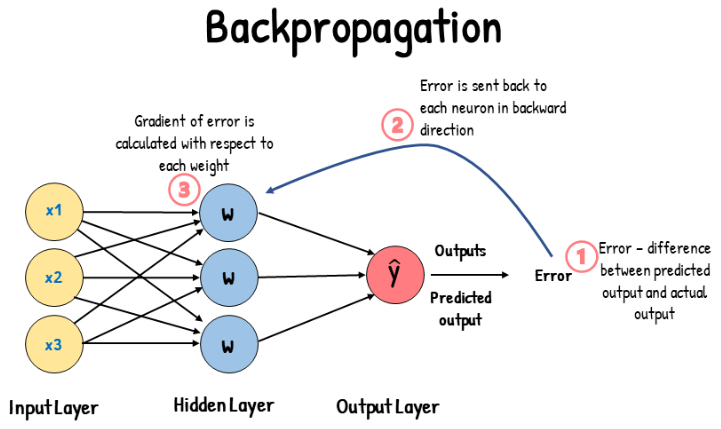
\includegraphics[width=0.85\linewidth]{WhatIsBackpropagation.png}
        \end{center}
    \end{figure}


\end{frame}

\begin{frame}
    \frametitle{Training: Backpropagation}
    \begin{itemize}
        \item \textbf{Calculate the output layer error: }Error of output layer:
        \[E_2 = A_2-Y\]
        \item \textbf{Calculate the gradient of the loss function with respect to $Z_2$: }The gradient of output layer:
        \[\delta_2 = E_2*g'(Z_2)\]
        \item \textbf{Calculate the gradient of hidden layer with loss function respect to $Z1$}The gradient of hidden layer:
        \[
            \delta_1 = \delta_1 W_2^t \cdot f'(Z_1), \quad f'(x) = 
            \begin{cases}
            1 & \text{if } x > 0, \\
            0 & \text{if } x \leq 0.
            \end{cases}
        \]

        \item \textbf{update the Weight and Biases: }
        \[W_2 = W_2 - \eta A_1^T \delta_2 ,\quad b_2 = b_2 - \eta \sum \delta_2,\quad W_1= W_1 - \eta X^T \delta_1,\quad b_1 = b_1 - \eta\sum \delta_1\]
    \end{itemize}

    
\end{frame}

\begin{frame}
    \frametitle{Evaluating: Loss Fuction-BCE}
    \begin{itemize}

        \item Binary Cross-Entropy Loss: Binary Cross-Entropy Loss is commonly used for binary classification problems. It measures the performance of a classification model whose output is a probability value between 0 and 1.    
            \[
              E = -\left[\quad y * \log(p) + (1 - y) * \log(1 - p) \quad\right]
            \]

        \item Mean Squared Error (MSE) Loss  : It measures the average squared difference between the actual and predicted values.
            \[
                BCE_{\textbf{avg}} = - \frac{1}{N} \sum i = 1^N \left[\quad y_i * \log(p_i) + (1 - y_i) * \log(1 - p_i) \quad\right]
            \]
        \item Categorical Cross-Entropy Loss(CCE) :It measures the performance of a classification model whose output is a probability distribution over multiple classes. 
            \[
            \frac{\partial BCE }{\partial p}  \quad=\quad \frac{p-y }{p(1-p)} \]
    \end{itemize}
\end{frame}

\begin{frame}
    \frametitle{ Loss Fuction-BCE}
   \begin{figure}
            \begin{center}
                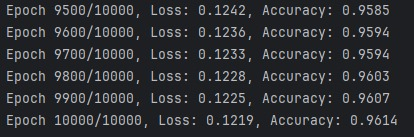
\includegraphics[width=1\linewidth]{BCE.jpg}
                \caption{Training \textbf{BCE} Loss Epochs }
                \label{fig:modelE}
            \end{center}
        
    \end{figure}
\end{frame}

\begin{frame}
    \frametitle{Evaluating: Loss Fuction-MSE}
    Mean Squared Error (MSE) Loss: 
    It measures the average squared difference between the actual and predicted values. 
    \vspace{0.5cm}
    \begin{itemize}

        \item \textbf{he Mean Squared Error Loss for a single sample:}
        \[
            MSE = (y - y')^2
        \]

        \item \textbf{he Mean Squared Error Loss for batch samples is:}
        \[
        MSE_{\textbf{avg}}= \frac{1}{N} \sum i = 1^N (y_i - y'_i)^2
        \]
        \item \textbf{The gradient of MSE:}
       \[
       \frac{\partial MSE}{\partial y'} =  2(y-y')^2
       \]
    \end{itemize}
\end{frame}

\begin{frame}
    \frametitle{ Loss Fuction-MSE}
   \begin{figure}
            \begin{center}
                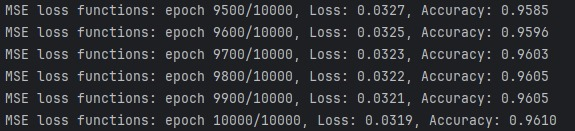
\includegraphics[width=1\linewidth]{MSE.jpg}
                \caption{Training \textbf{MSE} Loss Epochs }
                \label{fig:modelE}
            \end{center}
        
    \end{figure}
\end{frame}

\begin{frame}
    \frametitle{Evaluating: Loss Fuction-CCE}
    Categorical Cross-Entropy Loss(CCE): It measures the performance of a classification 
    model whose output is a probability distribution over multiple classes. 
    \vspace{0.5cm}

    \begin{itemize}

        \item  \textbf{Categorical Cross-Entropy Loss for a single sample is} 
        \[
            CCE = - \sum_{c=1}^{c} y_\text{c} * log(p_\text{c})
        \]

        \item \textbf{Categorical Cross-Entropy Loss for batch samples is }
        
\[
CCE_{\text{avg}} = - \frac{1}{N} \sum_{i=1}^{N\sum_{c=1}^{C}}  y_{ic} * \log(p_{ic})
\]
        
        \item \textbf{The gradient of CCE:}
       \[
       \frac{\partial CCE}{P_c} =  p_c - y_c
       \]
    \end{itemize}


\end{frame}

\begin{frame}
    \frametitle{ Loss Fuction-CCE}
   \begin{figure}
            \begin{center}
                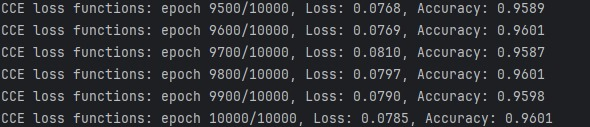
\includegraphics[width=1\linewidth]{CCE.jpg}
                \caption{Training \textbf{CCE} Loss Epochs }
                \label{fig:modelE}
            \end{center}
        
    \end{figure}
\end{frame}

\begin{frame}
    \frametitle{Model Evaluating and Testing}

    The model shows effective learning, with a consistent decrease in loss and a steady increase in accuracy over epochs,
     reaching \textbf{0.9565}. This indicates improved performance and gradual stabilization,
     with diminishing loss reductions in further training.
   \begin{figure}[h]
        \begin{minipage}[t]{0.35\linewidth}
            \begin{flushleft}
                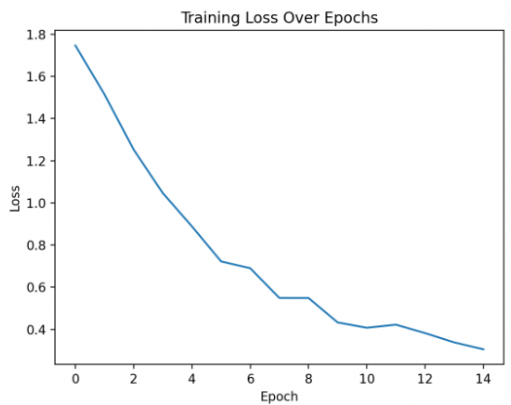
\includegraphics[width=\linewidth]{LossFunction.png}
                \caption{Training Loss Over Epochs }
                \label{fig:modelE}
            \end{flushleft}
        \end{minipage}
        \hfill
        \begin{minipage}[t]{0.5\linewidth}
            \begin{flushright}
                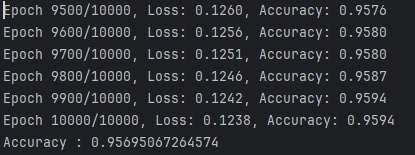
\includegraphics[width=\linewidth]{modelE.jpg}
                \caption{Accuracy Over Epochs}
                \label{fig:modelE}
            \end{flushright}
        \end{minipage}
    \end{figure}
    


    


\end{frame}



%Conclusion section
\begin{frame}{Conclusion}
    \frametitle{Conclusion}
    Our spam email detection model leverages cutting-edge techniques, 
    combining Multi-Layer Perceptron (MLP) or 
    Convolutional Neural Network (CNN) 
    architectures with the integration of nonlinear systems equations into backpropagation 
    and loss function calculations. This advanced approach enables the model to capture intricate patterns in email data, ensuring precise spam detection while adapting to evolving threats. Preprocessing steps such as tokenization, one-hot encoding, and token embedding streamline data handling, enhancing efficiency. By uniting these innovations, our system achieves exceptional accuracy, computational efficiency, and robustness, providing users with a cleaner, more secure inbox experience.
    
\end{frame}

\section{Thank You}








\end{document}